\section*{Задача 3.1}
Реализовать решение СЛАУ с помощью LU разложения и LU разложения по схеме частичного выбора. Решить систему небольшой размерности с возмущенной матрицей обоими методами, оценить погрешность и сравнить с теоретической оценкой. Проанализировать поведение  методов с ростом числа уравнений.

$A_{ij} = \arctan(0.1 (10i + j + 1)).$

\subsection*{Решение}
Напишим функцию создания матрицы размера m:
\begin{verbatim}
def init_matr(m):
    matr = np.zeros((m, m))
    for i in range(m):
        for j in range(m):
            matr[i][j] = np.arctan(0.1 * (10 * i + j + 1))
    return matr
\end{verbatim}

1. Реализуем метод решения СЛАУ с помощью LU разложения по схеме единственного деления, модифицирующий исходную матрицу A.
\begin{verbatim}
def LU(A) -> np.array:
    lu = A.copy()
    for i in range(1, A.shape[0]):
        for j in range(0, i):
            mu = lu[i, j] / lu [j, j]
            mask = np.ones_like(lu[j, :])
            mask[:j] = 0
            # print(lu[j, :] * mask)
            lu[i, :] -= mu * (lu[j, :] * mask)
            lu[i, j] = mu
    return lu

def solve(A, b):
    lu = LU(A)
    l = np.tril(lu, -1) + np.eye(lu.shape[0])
    u = np.triu(lu)
    # print(l)
    # print(u)
    y = np.linalg.inv(l).dot(b)
    x = np.linalg.inv(u).dot(y)
    # return l, u
    return x
\end{verbatim}

Убедимся в работоспособности метода:
\begin{verbatim}
solve(A, b)

array([[22. , 22. , 22.00000001, 22. , 22. ]])
\end{verbatim}

2. Реализуем метод решения СЛАУ с помощью LU разложения по схеме частичного выбора в виде двух функций, одна из которых возвращает две матрицы – L и U, не модифицируя A, а вторая функция решает систему.
\begin{verbatim}
def Mimod(A, k, is_l):
    mi = np.eye(*A.shape)
    P = np.eye(*A.shape)
    mx = k + np.argmax(np.abs(A[k:, k]))
    P[[k, mx]] = P[[mx, k]]
    A = P.dot(A)
    for i in range(k + 1, A.shape[1]):
        mi[i, k] = A[i, k] / A[k, k]
        if not is_l:
            mi[i, k] *= -1
    return mi, P

def LUmod(A):
    U = A.copy()
    L = np.eye(*A.shape)
    M = np.eye(*A.shape)
    for j in range(0, A.shape[1] - 1):
        mi, pi = Mimod(U, j, False)
        mii, pii = Mimod(U, j, True)
        U = mi.dot(pi).dot(U)
        L = L.dot(pii).dot(mii)
    return L, U

def solvemod(A, b):
    L, U = LUmod(A)
    y = np.linalg.inv(L) @ b
    x = np.linalg.inv(U) @ y
    return x
\end{verbatim}

Убедимся в работоспособности метода:
\begin{verbatim}
solve(A, b)

array([[22. , 21.99999999, 22.00000002, 21.99999998, 22. ]])
\end{verbatim}

3. Решим систему  $A^*x = b$, размера 5 x 5, двумя методами. $A^*$ зададим как $A$ и к одному элементу прибавим $10^{-3}$  
\begin{verbatim}
A_star  = A.copy()
A_star[3, 3] += 0.001
x1 = solve(A_star, b)
x2 = solvemod(A_star, b)
\end{verbatim}

4. Вычислим погрешности и сравним с теоретической оценкой.
\begin{verbatim}
Dx1 = np.linalg.norm(x_root - x1)
Dx2 = np.linalg.norm(x_root - x2)
DA = np.linalg.norm(A - A_star)
dx1 = Dx1 / np.linalg.norm(x_root)
dx2 = Dx2 / np.linalg.norm(x_root)
dA = DA / np.linalg.norm(A)
condA = np.linalg.norm(A) * np.linalg.norm(np.linalg.inv(A))
d_hat = condA * DA
print(f'{dx1 = }')
print(f'{dx2 = }')
print(f'Теоретическая оценка: {d_hat}')


dx1 = 0.8568133536857635
dx2 = 0.8568133536692295
Теоретическая оценка: 56493.659253590085
\end{verbatim}

Погрешность решений полученых обоими методами находится в пределах теоретической оценки.

5. Решим систему обоими методами для матриц большей размерности. Построим на одном графике погрешности обоих методов как функций, зависящих от $n$.

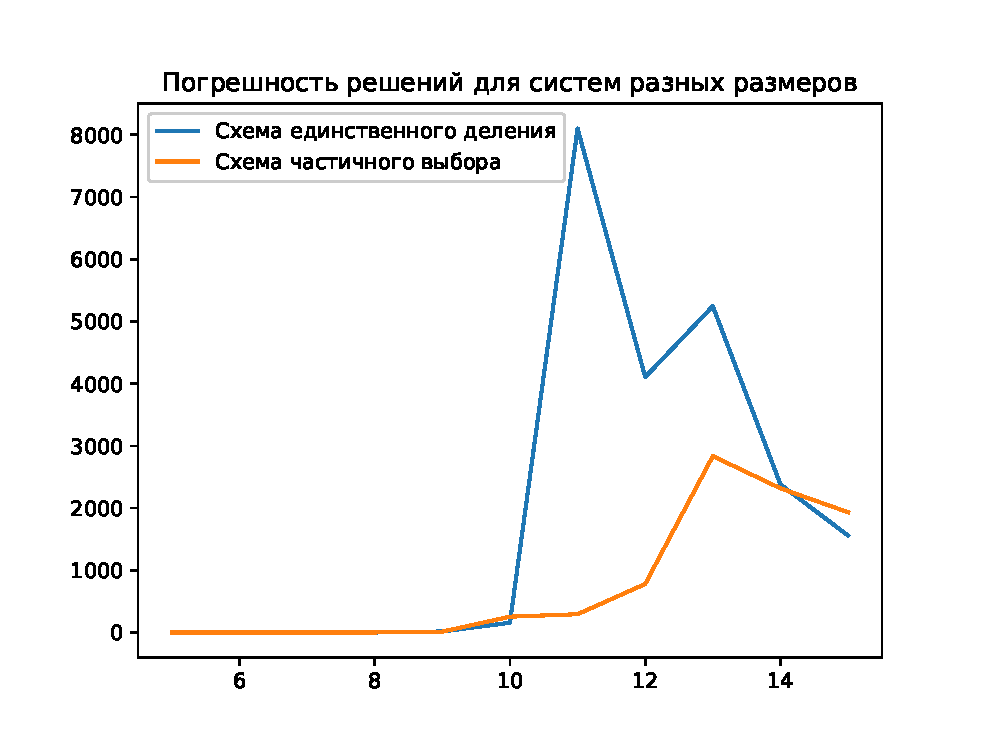
\includegraphics[width=15cm]{311.eps}

Из графиков видно, что погрешность прямых методов возрастает с размерами системы, при этом метод частичного выбора дает более точный результат.
